\section{TCP versions}

\subsection{TCP Tahoe}
One of the first protocols, very basic. It uses the Slow Start Phase and 
AIMD, but it only relies on timeouts to detect losses, so no fast retransmit nor 
fast recovery (it doesn't check for dupacks). At every loss, it always restart 
from 1.

\paragraph*{Characteristics}
\begin{itemize}
  \item Standard TCP functions
  \item ``Slow'' start
  \item Congestion control: AIMD, only timeouts to detect losses (no dupacks)
\end{itemize}

\begin{figure}[h]
  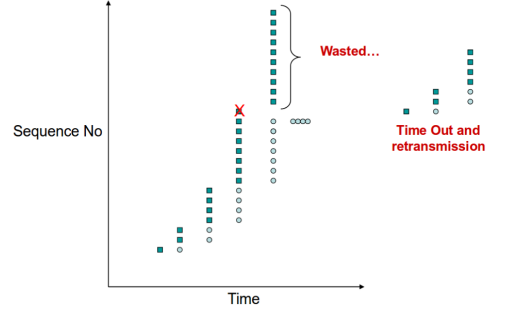
\includegraphics[scale=0.8]{tahoe}
  \caption[TCP Tahoe]{TCP Tahoe uses only timeouts to detect losses}
\end{figure}

\subsection{TCP Reno}
\paragraph*{Characteristics}
\begin{itemize}
  \item Fast Retransmit/Fast Recovery (3 dupAcks to recover one packet loss)
  \item TCP Reno can recover from one packet loss without having a time out
\end{itemize}

\begin{figure}[h]
  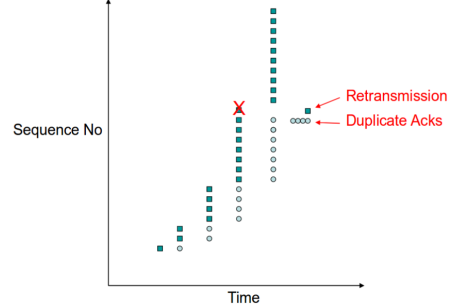
\includegraphics[scale=0.8]{fast_retransmit}
  \caption[TCP Reno 1]{TCP Reno - Fast Retransmission}
\end{figure}

\begin{figure}[h]
  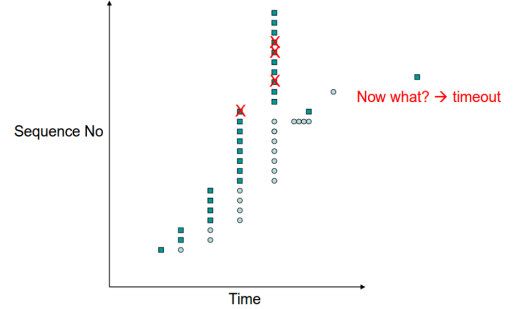
\includegraphics[scale=0.8]{reno}
  \caption[TCP Reno 2]{TCP Reno - more than one packet loss}
\end{figure}

\subsubsection{TCP New Reno}
TCP New Reno introduces partial ACKs to recover more packets without the use of
timeouts.
\begin{figure}[h]
  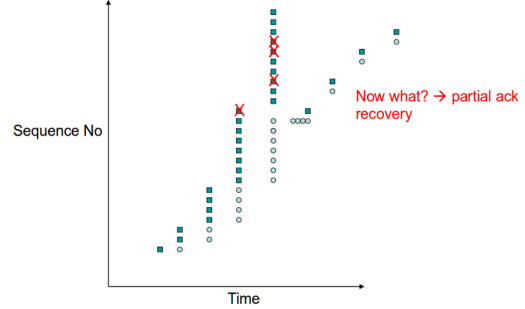
\includegraphics[scale=0.8]{partial_acks}
  \caption[TCP New Reno]{TCP New Reno - partial ACKs}
\end{figure}

\subsection{TCP SACK}
SACK means \textit{Selective acknowledgment}. This means that all ACKs are a
little bigger but carry more information, they can give the sender the complete 
picture.

Returning ACKs declares which packets (even non contiguous) were received.
All non-received packets can be retransmitted and so it recovers from multiple
losses in just one RTT.
\begin{figure}[h]
  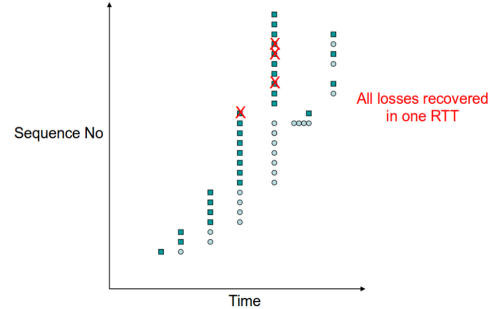
\includegraphics[scale=0.8]{sack}
  \caption[TCP SACK]{TCP SACK - Recovery from multiple losses in just one RTT}
\end{figure}
